\subsection{UC2: Configurazione della connessione tra rete bayesiana e sorgente dati}
\begin{figure} [H]
	\centering
	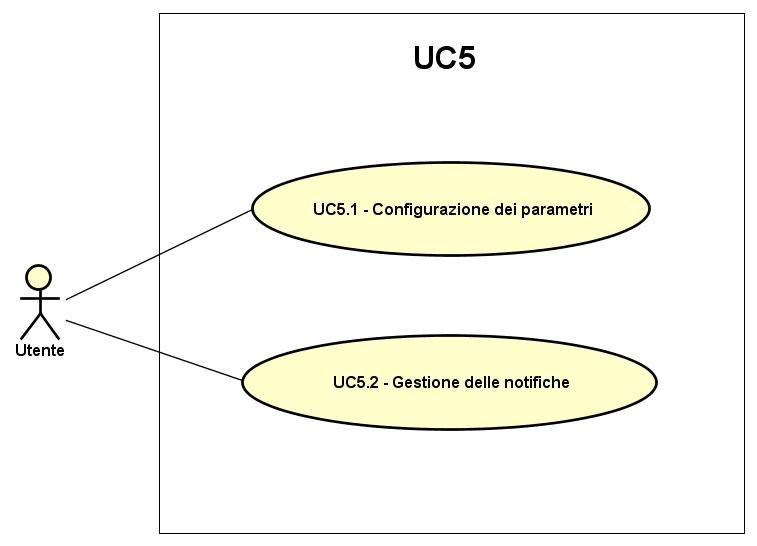
\includegraphics[scale=0.45]{Img/UC5}
	\caption{UC2: Configurazione della connessione tra rete bayesiana e sorgente dati}\label{}
\end{figure}
\begin{itemize}
	\item \textbf{Attori}: Utente;
	\item \textbf{Descrizione}: L'attore configura la connessione dei nodi della rete ai rispettivi flussi di dati provenienti dalla \gl{sorgente dati};
	\item \textbf{Precondizione}: É stata creata o caricata una rete bayesiana adeguata; Grafana riceve correttamente informazioni dalla sorgente dati;
	\item \textbf{Flusso principale degli eventi}:
	\begin{itemize}
		\item Gestione della connessione tra un nodo ed un flusso di dati (UC2.1);
		\item Salvataggio della configurazione attuale (UC2.2);
		\item Caricamento di una configurazione salvata (UC2.3).
	\end{itemize}
	\item \textbf{Postcondizione}: La connessione tra la rete bayesiana e la sorgente dati é configurata correttamente.
\end{itemize}

\subsection{UC2.1: Gestione della connessione tra un nodo ed un flusso di dati}
\begin{figure} [H]
	\centering
	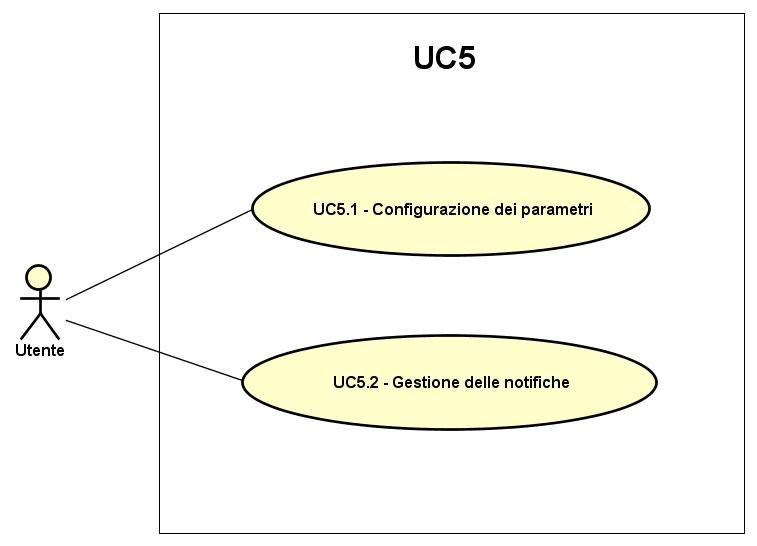
\includegraphics[scale=0.45]{Img/UC5}
	\caption{UC2.1: Gestione della connessione tra un nodo ed un flusso di dati}\label{}
\end{figure}
\begin{itemize}
	\item \textbf{Attori}: Utente;
	\item \textbf{Descrizione}: L'attore modifica il modo in cui un nodo é connesso ad un flusso di dati;
	\item \textbf{Precondizione}: L'attore ha selezionato un nodo della rete bayesiana;
	\item \textbf{Flusso principale degli eventi}:
	\begin{itemize}
		\item Connessione di un nodo ad un flusso di dati (UC2.1.1);
		\item Disconnessione di un nodo ad un flusso di dati (UC2.1.2);
		\item Modifica del flusso di dati connesso ad un nodo (UC2.1.3).
	\end{itemize}
	\item \textbf{Postcondizione}: Il nodo selezionato é connesso al, oppure disconnesso dal, flusso di dati designato.
\end{itemize}